\documentclass{article}
\usepackage[utf8]{inputenc}
\usepackage{indentfirst}
\usepackage{titling}
\usepackage{geometry}
\usepackage{graphicx}
\graphicspath{ {./Images/} }
\usepackage[shortlabels]{enumitem}
\usepackage{fancyhdr}
\usepackage{ulem}
\usepackage[dvipsnames]{xcolor}
\usepackage{amssymb}
\usepackage{listings}
\usepackage{color}

\definecolor{dkgreen}{rgb}{0,0.6,0}
\definecolor{gray}{rgb}{0.5,0.5,0.5}
\definecolor{mauve}{rgb}{0.58,0,0.82}

\lstset{frame=tb,
  language=Java,
  aboveskip=3mm,
  belowskip=3mm,
  showstringspaces=false,
  columns=flexible,
  basicstyle={\small\ttfamily},
  numbers=none,
  numberstyle=\tiny\color{gray},
  keywordstyle=\color{blue},
  commentstyle=\color{dkgreen},
  stringstyle=\color{mauve},
  breaklines=true,
  breakatwhitespace=true,
  tabsize=3
}

\def\ojoin{\setbox0=\hbox{$\bowtie$}%
  \rule[-.02ex]{.25em}{.4pt}\llap{\rule[\ht0]{.25em}{.4pt}}}
\def\leftouterjoin{\mathbin{\ojoin\mkern-5.8mu\bowtie}}
\def\rightouterjoin{\mathbin{\bowtie\mkern-5.8mu\ojoin}}
\def\fullouterjoin{\mathbin{\ojoin\mkern-5.8mu\bowtie\mkern-5.8mu\ojoin}}

\renewcommand\maketitlehooka{\null\mbox{}\vfill} %para centralizar verticalmente
\renewcommand\maketitlehookd{\vfill\null}
\pagestyle{fancy}
\fancyhf{}
\rfoot{\thepage}
\lfoot{ 
\includegraphics[scale=0.01]{UA.jpg} José Mendes 107188 LEI}
\geometry{
  a4paper,
  headheight=4cm,
  top=5.5cm,
  bottom=4.5cm,
  footskip=4cm
}


\title{Inteligência Artificial}
\author{José Mendes 107188}
\date{2023/2024}

\begin{document}


\begin{titlepage}
    \maketitle
    \begin{center}
        
\includegraphics[scale=0.4]{UA.png}
    \end{center}
    \thispagestyle{empty} %remove o count da pagina
\end{titlepage}

\pagebreak

\section{Noções de Programação Declarativa}

\subsection{Programação Declarativa}

A Programação Declarativa abstrai-se da implementação, focando-se
apenas na descrição do que se pretende fazer, enquanto faz uso de dois
paradigmas:
\begin{itemize}
  \item \textbf{Programação Funcional}, baseado em funções/calculo-lambda, a entidade central é a função;
  \item \textbf{Programação em Lógica}, baseado em lógica de primeira ordem, a entidade central é o predicado;
\end{itemize}


\subsection{Paradigma Imperativo}

O fluxo de operações é especialmente sequenciado de operações com
foco na forma como as tarefas são executadas (\textbf{instrução}). Podemos \textbf{alterar
o conteúdo em memória} e ainda (instruções de afetação/atribuição) e ainda
\textbf{realizar análise de casos} (if-then-else, switch/case, \dots), \textbf{processamento
iterativo} (while, repeat, for, \dots) e ter associados \textbf{sub-programas} (procedimentos,
funções).

\begin{flushleft}
\textbf{Exemplo:} SQL é uma linguagem declarativa, uma vez que nos seus comandos apenas descrevemos o que queremos obter.
Assim, o programador é abstraído da forma como as operações são executadas na prática, ficando essa tarefa a cargo
do compilador.
\end{flushleft}

\subsection{Paradigma Declarativo}

\begin{center}
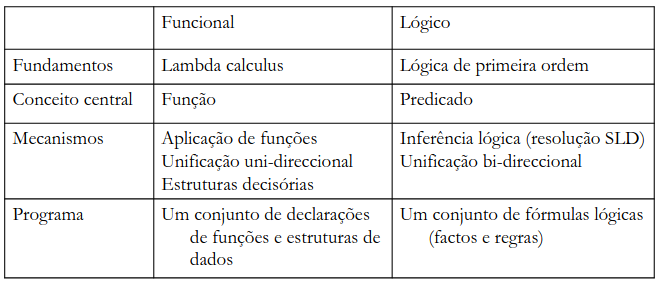
\includegraphics[scale=0.5]{1}
\end{center}

A sua origem data da segunda metade do século XX, mas ainda hoje é amplamente usada e
até está em crescimento em áreas como a Inteligência Artifical.

\pagebreak

\subsection{Programação Funcional}

Possibilidade de definir funções localmente e sem nome. Por exemplo as
funções lambda presentes em Lisp e Python.

\subsection{Programação em Lógica}

Um programa é uma teoria sobre um domínio. Por exemplo, temos
\textbf{socrates é um homem}, $homem(socrates)$ e, um \textbf{homem é mortal}, $homem(X) :- \hspace{1mm} mortal(X)$.
Se perguntarmos se \textbf{socrates é mortal}, $mortal(socrates)$, a resposta é \uline{sim}.

\subsection{Atitude do programador}

A programação declarativa, dada a sua elevada expressividade, é pouco
compatível com aproximações empíricas (ou seja, tentativa e erro) à programação.
Primeiro é preciso pensar bem na estrutura do problema antes de começar a teclar.

\vspace{2mm}

\begin{flushleft}
  \textbf{Passos a seguir:} Perceber o problema $\rightarrow$ Desenhar o programa $\rightarrow$
  Escrevê-lo $\rightarrow$ Rever e testar
\end{flushleft}

\subsection{Características da Programação Funcional}

\begin{itemize}
  \item A entidade central é a função;
  \item A noção de função é diretamete herdada da matemática (ao contrário das
  linguagens imperativas, que pode ser muito diferente);
  \item A estrutura de controlo fundamental é a "aplicação de funções";
  \item A noção de "tipo da função" captura a noção matemática de
  domínio (de entrada e saída);
  \item Os elementos do domínio de entrada e saída podem ser funções;
\end{itemize}

\subsection{Função}

Tem valores de entrada (domínio) e valores de saída (contradomínio).

\begin{center}
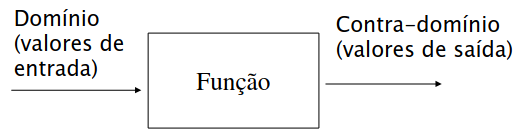
\includegraphics[scale=0.4]{2}
\end{center}

\subsection{Programação em Lógica}

Um programa numa linguagem baseada em lógica representa uma teoria sobre um
problems. Um programa é uma sequência de frases ou fórmulas representando
\textbf{factos} (informação sobre objetos do problema/domínio de aplicação) e \textbf{regras}
(leis gerais sobre esse problema/domínio). Implicitamente as frases estão reunidas
nume grande conjunção, e cada frase está universalmente quantificada. Portanto,
\textbf{programação declarativa}.

\pagebreak

\section{Programação ao estilo funcional em Python}

\subsection{Python}

Criada no final dos anos 90, é uma linguagem de programação interpretada,
iterativa, portável, funcional, orientada a objetos e de implementação aberta.
Tem como principais objetivos: simplicidade sem prejuizo da utilidade,
programação modular, legibilidade, desenvolvimento rápido, facilidade de integração,
nomeadamente com outras linguagens. Apresenta-se como uma linguagem \textbf{multi-paradigma}:
\begin{itemize}
  \item \textbf{Programação funcional:} Expressões lambda, funções de ordem superior,
  listas com sintaxe simples, iteradores, \dots
  \item \textbf{Programação OO:} Classes, objetos, métodos, herança, \dots
  \item \textbf{Programação imperativa/modular:} Atribuição, sequências,
  condicionais, ciclos, \dots
\end{itemize}

\subsubsection{Python vs Java}

Comparativamente ao JAVA revela-se menos consisa porque os espaços são sintaticamente
relevantes e o código, não compilado para código nativo (interpretado), demora mais tempo a
executar (diferença residual), no entanto apresenta uma maior facilidade de desenvolvimento e
legibilidade.

\subsubsection{Áreas de aplicação}

As principais áreas de aplicação são: interligação de sistemas, aplicações gráficas,
aplicações para bases de dados, multimédia, internet protocol/web e
robótica e inteligência artificial.

\subsection{Dados, ou "objetos"}

\begin{flushleft}
  \textbf{Objeto:} no contexto de Pyhton, esta designação é
  aplicada a qualquer dado que possa ser armazenado
  numa variável, ou passado como parâmetro a uma
  função.
\end{flushleft}

Cada objeto é caracterizado por uma identidade/referência (identifica a posição
de memória onde está armazenado), um tipo e um valor. Alguns tipos de
objetos podem ter atributos e métodos, outros (classes) podem ter
sub-tipos (sub-classes).

\begin{center}
  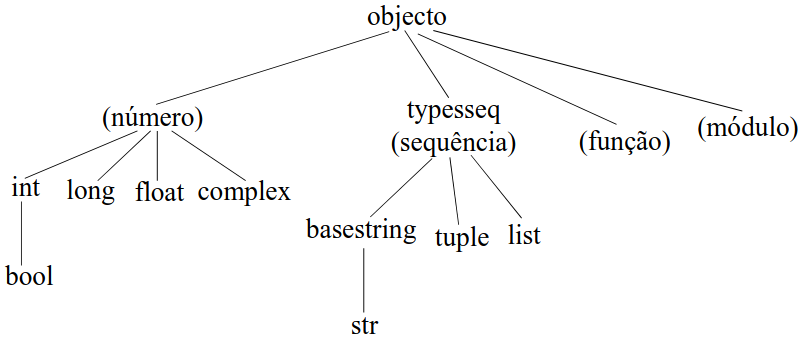
\includegraphics[scale=0.3]{3}
\end{center}

Alguns destes são imutáveis, como as \textbf{str} e \textbf{tuple}. Para determinar o tipo de um objeto utiliza-se a função pré-definida \textbf{type()}.

\pagebreak

\subsection{Variáveis}

As variáveis guardam objetos, mas não são declaradas (inicializadas apenas) nem têm tipos
associados (o tipo é do objeto!). Praticamente tudo pode ser atribuido a uma variável, incluindo
funções, módulos e classes. Similar as linguagens imperativas, e ao contrário das
funcionais, o valor de uma variável pode ser alterado. Não se pode ler o valor de uma variável
se este não tiver sido previamente inicializado.

\subsection{Intrução de atribuição}

Tal como é habitual na programação imperativa, e ao
contrário do habitual na programação declarativa,
Python possui instrução de atribuição.

\begin{flushleft}
  \textbf{Exemplo:}
  \begin{lstlisting}
    n = 10
    a = b = c = 0
    x = 7.25
    cad = "cadeia"
    t = (n, x)
    l = [1, 2, 'quatro', 5.0]
  \end{lstlisting}
\end{flushleft}

Pode user a operação de atribuição para decompor estruturas:
\begin{lstlisting}
  triplo = (1, 2, 3)
  (i, j, k) = triplo
\end{lstlisting}

\subsection{Operadores}

Operadores comuns matemáticos e lógicos. É importante saber que objetos de
tipos diferentes nunca são iguais (exceto os diferentes tipos de números).

\subsubsection{Operadores lógicos}

Na conjunção e disjunção, o segundo elemento só é avaliado de for necessário para determinar
o resultado.

\begin{lstlisting}
  if False and a: # a nao e avaliado
    ...

  if True or a: # a nao e avaliado
    ...
\end{lstlisting}

\pagebreak

\subsection{Acesso a sequências}

Os elementos das sequências são acedidos
através de índices inteiros consecutivos (primeiro elemento tem índice 0).

\vspace{2mm}

É possível extrair “fatias” das sequências. A indexação é circular, pelo que podemos aceder a
índices negativos.

\begin{lstlisting}
  # [inf:sup] retorna a sequencia entre os indices inf e sup-1 (uma opia da lista)

  # Para fazer uma copia integral da lista usa-se [:]
\end{lstlisting}

\begin{flushleft}
  \textbf{Detalhe importante:}  instrução de atribuição, em vez de copiar valores, limita-se
  a associar um dado identificador a um dado objecto. Desta forma, a atribuição
  da variável x a uma variável y, apenas tem como resultado associar y
  ao mesmo objecto que x já estava associada. No caso dos objetos
  mútaveis, temos de ter cuidado:

  \begin{lstlisting}
    a = [1, 2, 3]
    b = a
    b[1:2] = []
    print(a) # [1, 3]
  \end{lstlisting}
\end{flushleft}

\subsection{Definição de funções}

Funções sem return, retornam None, são também conhecidas como procedimentos. As funções podem
ser recursivas e são objetos do tipo \textbf{function}.

\vspace{2mm}

Os parâmetros são passados às funções segundo um mecânismo "passagem por valor"
("call by value"). \uline{Os parâmetros são passados por referêcia, não cópias!}. 

\vspace{2mm}

Se atribuirmos um novo objeto a uma variável passada por
parâmetro, essa atribuição ocorre apenas no espaço de nomes da função (imagem à
esquerda). Se modificarmos um objeto passado por parâmetro (por
exemplo, apagar um elemento de uma lista), isto não altera a
referência do objeto, e portanto vai permanecer após o
retorno da função (imagem à direita).

\begin{center}
  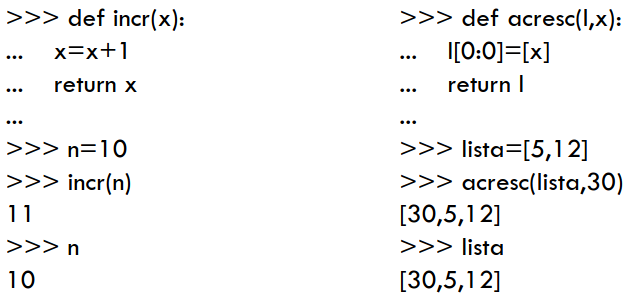
\includegraphics[scale=0.3]{4}
\end{center}

O problema anterior resolve-se trabalhando sobre uma cópia local,
no caso de uma lista l, podemos usar l[:], que dá uma cópia integral.

\pagebreak

Podemos passar parâmetros com valores por defeito, podendo se, na chamada,
omitir alguns parâmetros.

\begin{lstlisting}
  def abc(arg1, arg2=True, arg3=None):
    ...
  # Quando so queremos passar um dos args por defeito devemos indicar o seu nome
  abc(1, arg3=3)
\end{lstlisting}

\subsection{Funções Recursivas}

\begin{lstlisting}
  # devolve factorial de um numero n
  def factorial(n):
    if n==0:
      return 1
    if n>0:
      return n*factorial(n-1)

  # devolve o comprimento de uma lista
    def comprimento(lista):
      if lista==[]:
        return 0
      return 1+comprimento(lista[1:])
\end{lstlisting}

\begin{flushleft}
  Esta última função, vai funcionar da seguinte forma:
\end{flushleft}

\begin{lstlisting}
  comprimento([1, 2, 3])
  =
  1 + comprimento([2, 3])
  =
  1 + (1 + comprimento([3]))
  =
  1 + (1 + (1 + comprimento([])))
  =
  1 + (1 + (1 + 0))
  =
  3
\end{lstlisting}

\begin{lstlisting}
  # verifica se um elemento e membro de uma lista
  def membro(x,lista):
    if l==[]:
      return False
    return (lista[0]==x) or membro(x,lista[1:])
\end{lstlisting}

\pagebreak

\begin{lstlisting}

  # devolve uma lista com os elementos da lista de entrada por ordem inversa
  def inverter(lista):
    if lista==[]:
      return []
    inv = inverter(lista[1:])
    inv[len(inv):] = [lista[0]]
    return inv
\end{lstlisting}

\subsection{Expressões lambda}

São \textbf{expressões cujo valor é uma função}. Funções que recebem expressões lambda como
entrada e as retornam como saída chamam-se funções de ordem superior. Exemplo:

\begin{lstlisting}
  lambda x: x*x

  # Pode ser atribuida a uma variavel
  m = lambda x,y: math.sqrt(x**2 + y**2)
  m(1, 2) # 2.23606797749979
\end{lstlisting}

Como qualquer objeto, uma expressão lambda pode ser passada como:

\begin{lstlisting}
  # Tendo uma func h que produz f(x)*X
  def h(f, x): return f(x)*x

  # Para usar:
  h(lambda x: x+1, 7) # 56
\end{lstlisting}

Podem ser produzidas por outras funções:

\begin{lstlisting}
  def faz_incrementador(n):
    return lambda x: x+n

  # Para usar:
  f = faz_incrementador(1)
  f(10) # 11
\end{lstlisting}

As expressões lambda são tembém conhecidas como \uline{expressões funcionais}.
As funções que recebem estas expressões como entrada e/ou produzem expressões
lambda como saída chamam-se \uline{funções de ordem superior}.

\begin{flushleft}
  \textbf{Nota importante:} As expressões lambda só são
  úteis enquanto são simples. Uma função
  complexa merece ser escrita de forma clara
  numa definição (def) à parte.
\end{flushleft}

\pagebreak

\subsection{Aplicar uma função a uma lista}

Para tal podemos usar a função \textbf{map()}, predefinida em Python,
retorna um iterador que pode ser convertido numa lista. Esta função é
equivalente a:

\begin{lstlisting}
  def aplicar(funcao, lista):
    if lista==[]:
      return []
    return [funcao(lista[0])] + aplicar(funcao, lista[1:])
\end{lstlisting}

\subsection{Filtrar uma lista}

Para tal podemos usar a função \textbf{filter()}, predefinida em Python,
retorna um iterador que pode ser convertido numa lista. Esta função é
equivalente a:

\begin{lstlisting}
  def filtrar(funcao, lista):
    if lista==[]:
      return []
    if funcao(lista[0]):
      return [lista[0]] + filtrar(funcao, lista[1:])
    return filtrar(funcao, lista[1:])
\end{lstlisting}

\subsection{Reduzir uma lista a um valor}

Muitos dos procedimentos aplicados a listas consistem em combinar a cabeça da lista com o
resultado da chamada recursiva sobre os restantes elementos, retornando um valor “neutro”
pré-definido para a lista vazia. Em Python, podemos usar a função \textbf{reduce()} da
biblioteca \textbf{functools}.

\begin{center}
  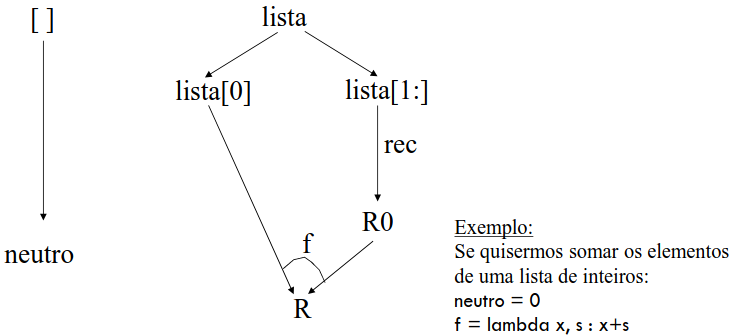
\includegraphics[scale=0.3]{5}
\end{center}

\begin{lstlisting}
  # Dada uma lista, uma func de combinacao e um elemento neutro
  def reduzir(lista, fcomb, neutro):
    if lista==[]:
      return neutro
    return fcomb(lista[0], reduzir(lista[1:], fcomb, neutro))
\end{lstlisting}

\pagebreak

\subsection{Listas por compreensão (list comprehension)}

São mecanismos compactos para processar os elementos de uma lista (alguns ou todos), podendo ser aplicadas
não só a estas como também a tuplos ou cadeias de caracteres (str), o resultado é uma lista. Podem funcionar com a
função pré-definida \textbf{map()} ou \textbf{filter()}.

\[<expr> \textbf{for} <var> \textbf{in} <seq> \textbf{if} <condition>\]

\begin{lstlisting}
  [x**2 for x in [2, 3, 4]] # Output: [4, 9, 16]
  map(lambda x: x**2, [2, 3, 4]) # Igual

  [x for x in [2, 3, 4] if x%2==0] # Output: [2, 4]
  filter(lambda x: x%2==0, [2, 3, 4]) # Igual
\end{lstlisting}

Dada uma lista de listas e uma função, podemos aplicar uma função
a cada um dos elementos das listas, retornando a concatenação
das listas resultantes.

\begin{lstlisting}
  [f(y) for x in lista for y in x]

  # Exemplo:
  lista = [[1, 2, 3], [4, 5, 6]]
  [x+1 for x in lista for y in x] # [2, 3, 4, 5, 6, 7]
\end{lstlisting}

\subsection{Classes}

Tal como nas restantes linguagens Orientadas a Objetos (OO), em Python uma classe define
um conjunto de objetos caracterizados por diversos atributos e métodos e organizam-se numa
hierarquia que permite a herança.

\begin{lstlisting}
  # sintaxe
  class <nome-classe>:
    <decl-1>
    ...
    <decl-n>
\end{lstlisting}

\begin{flushleft}
  \textbf{Nota:} Tal como acontece com as variáveis normais, também
  os atributos das classes \uline{não são declarados}. Os atributos são
  acessados através da notação "objeto.atributo". Podemos, em qualquer momento,
  criar um novo atributo para um objeto, bastando para isso atribuir-lhe um valor.
\end{flushleft}

Existe ainda classes derivadas/herança, que herdam os métodos e atributos da
classe mãe, sendo possível uma classe ter várias classes mães.

\pagebreak

\subsubsection{Métodos e atributos pré-definidos}

\begin{flushleft}
  \textbf{Métodos:}
  \begin{itemize}
    \item \textbf{\_\_init\_\_} - Construtor da classe;
    \item \textbf{\_\_str\_\_} - Conversão para cadeia de caracteres;
    \item \textbf{\_\_repr\_\_} - Representação em cadeia de caractéres
    que aparece na consola do interpretador;
  \end{itemize}

  \textbf{Atributos:}
  \begin{itemize}
    \item \textbf{\_\_class\_\_} - identifica a classe de um dado objecto
  \end{itemize}
\end{flushleft}

\subsubsection{list de Python é uma classe}

\begin{flushleft}
  Tem os seguintes métodos:
  \begin{itemize}
    \item \textbf{append(x)} - Adiciona x ao fim da lista;
    \item \textbf{extend(L)} - Adiciona os elementos da lista L ao fim da lista;
    \item \textbf{insert(i, x)} - Adiciona x na posição i da lista;
    \item \textbf{remove(x)} - Remove a primeira ocorrência de x na lista;
    \item \textbf{index(x)} - Devolve o índice da primeira ocorrência de x na lista;
    \item \textbf{sort()} - Ordena a lista (modifica a lista);
  \end{itemize}
\end{flushleft}

\section{Tópicos de Inteligência Artificial}

\subsection{Definição de "Inteligência"}

Segundo a sua definição lexical, \textbf{inteligência} é a capacidade de pensar, raciocionar, adquirir e
aplicar conhecimento. É o conjunto de capacidades superiores da mente.

\vspace{2mm}

O seu estudo envolve várias vertendes, desde a já referida aquisição, representação e
armazenamento de conhecimento, a geração de comportamento inteligente, a origem das
motivações, emoções e prioridades, como as perceções dão origem a entidades simbólicas,
como raciocionar sobre o passado, planear o futuro, como surge a ilusão, a crença, esperança,
amor \dots

\pagebreak

\subsection{Defunição de "Inteligência Artificial"}

É a disciplina que estuda as teoriaas e técnicas necessárias ao desenvolvimento
de "artefactos" inteligentes. Historicamente, estas vertententes resumem-se a quatro grandes abordagens, definidas por
Russel \& Norvig (1995).

\begin{center}
  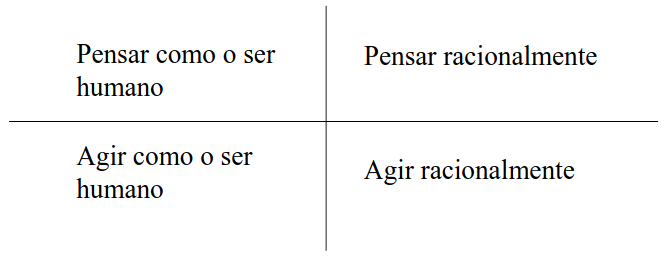
\includegraphics[scale=0.3]{6}
\end{center}

As \textbf{humanas} focam-se no ser humano, desenvolvendo uma ciência empírica, baseada na
hipótese e na experiência. Por outro lado, a \textbf{abordagem racional} envolve uma combinação de
matemática e engenharia.

\begin{flushleft}
  \textbf{Nota:} No início estava muito focada na imitação das capacidades do ser humano, no entanto, mais recentemente tem-se
  voltado mais para a racionalidade como referêcia. Atualmente é maioritariamente utilizada para a resolução de problemas concretos e pouco abrangentes, foncando-se
  na melhor utilização dos recursos de forma racional.
\end{flushleft}

\subsection{Definição de "Agente"}

Segundo o dicionário, pode ser uma entidade com poder ou autoridade para agir, ou
uma entidade que atua em representação de outrem.

\vspace{2mm}

\begin{flushleft}
  \textbf{Agente -} Definido como uma entidade com capacidade de obter informação sobre o seu ambiente
  (sensores) e de executar (atuadores) ações em função dessa informação por Russel e Norvig.
\end{flushleft}

\begin{center}
  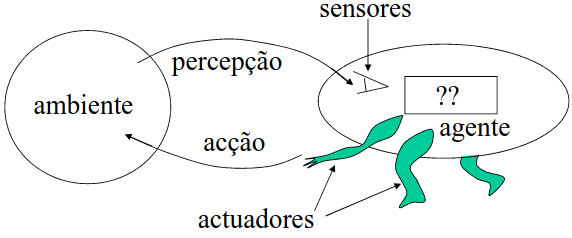
\includegraphics[scale=0.3]{7}
\end{center}

\pagebreak

\subsubsection{Exemplo de agentes}

\begin{center}
  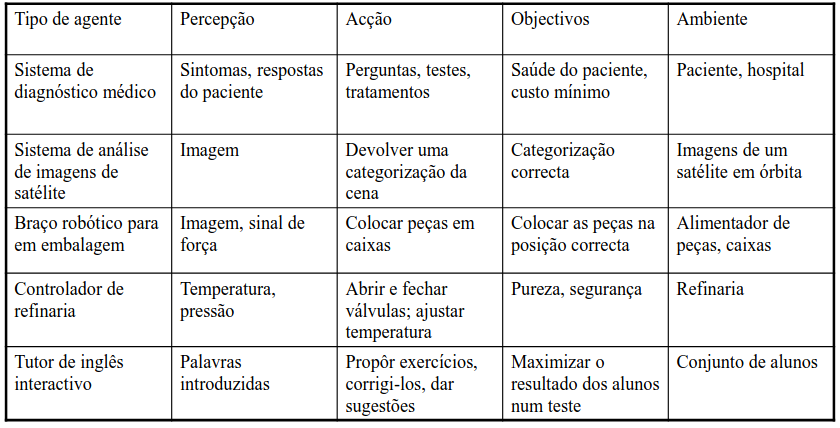
\includegraphics[scale=0.35]{8}
\end{center}

\subsection{Agir como o ser humano - Teste de Turing}

O \textbf{teste de Turing} (1950) pretendeu estebelecer a definição operacional para o comportamento
inteligente de nível humano, que consistia em submeter o artefacto a um interrogatório através
de um terminal de texto. Se o humano não conseguir concluir que está a interrogar uma
máquina, então conclui-se que o artefacto é inteligente.

\subsection{A "sala chinesa" de Searle}

Esta teoria foi refutada por \textbf{Searle}, um filósofo americano, com o argumento da \textbf{Sala Chinesa}.
Neste, descreveu o cenário de colocar um humano que não percebe chinês fechado dentro de
uma sala com um livro escrito na sua língua que ensine chinês a ser interrogado por outro
humano através de papéis passados por baixo da porta.

\vspace{2mm}

\textbf{Searle} defendeu que apesar de não perceber os papéis entregues por baixo da porta, o
humano iria conseguir traduzi-los através do livro e elaborar respostas. Fora da sala, o
interrogador iria ter a ilusão de que o interrogado sabia chinês. No entanto, nem o humano, nem
a sala, nem o livro percebem chinês. Logo, deduziu que não há qualquer compreensão de
chinês naquela sala. No entanto, podemos contra-argumentar que,
embora individualmente, os componentes do sistema não percebam chinês
(a sala, o humano, o livro, as folhas de papel), não compreendam chinês,
\textbf{o sistema no seu conjunto compreende chinês}.

\vspace{2mm}

Foi esta a premissa para a sua argumentação de que os computadores apenas fazem uso de
regras sintáticas para manipular o texto, sem ter qualquer entendimento do seu significado ou
semântica. Para ele a inteligência é um processo biológico, que apenas pode ser simulado
pelas máquinas, mas nunca adquirido.

\pagebreak

\subsection{Tipos e arquiteturas de agentes}

\begin{flushleft}
  \textbf{Tipos de agentes:}
  \begin{itemize}
    \item Reativo simples;
    \item Reativo com estado;
    \item Deliberativos orientados a objetivos;
    \item Deliberativos orientados por funções de utilidades;
  \end{itemize}

  \textbf{Arquiteturas de agentes:}
  \begin{itemize}
    \item Subsunção;
    \item Três torres;
    \item Três camadas;
    \item CARL;
  \end{itemize}
\end{flushleft}

\subsubsection{Agentes reativos: simples}

\begin{center}
  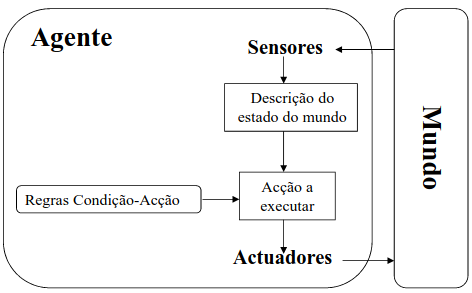
\includegraphics[scale=0.4]{9}
\end{center}

Também conhecidos por agentes de \textbf{estímulo-resposta} (ou "sistemas de produção"), este tipo de agente apresenta um
conjunto de sensores, através dos quais recebe uma perceção do estado do mundo, sobre a
qual aplica um conjunto de regras (regras de condição-ação, também conhecido
como "regras de situação-ação" ou "regras de produção") e executa as ações
correspondentes.

\begin{center}
  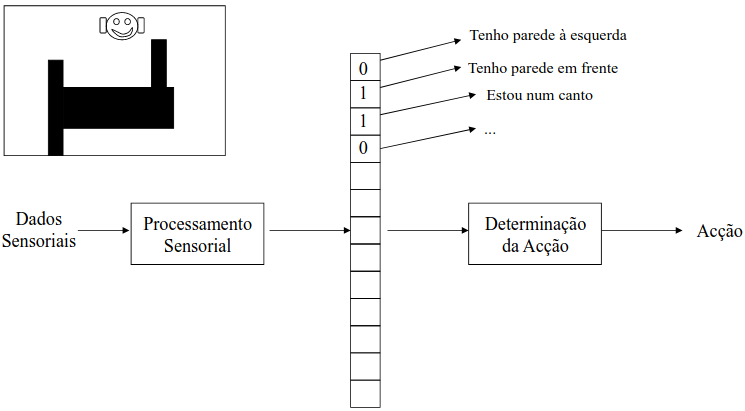
\includegraphics[scale=0.35]{10}
\end{center}

\pagebreak

\subsubsection{Agentes reativos: com estado interno}

\begin{center}
  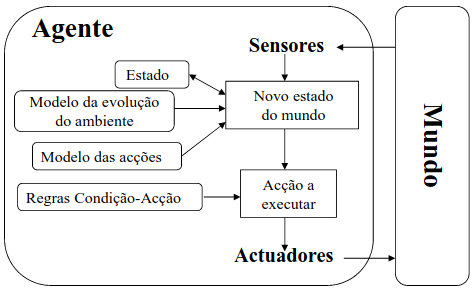
\includegraphics[scale=0.4]{11}
\end{center}

Funcionam de forma semelhante ao
anterior, mas para além dos sensores, fazem uso de um \textbf{estado interno} e do histórico de ações
anteriores para construir a perceção do estado do mundo.

\begin{center}
  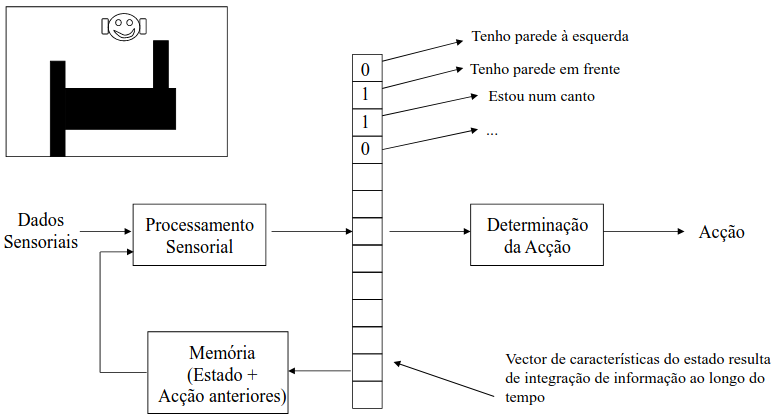
\includegraphics[scale=0.35]{12}
\end{center}


\subsubsection*{Sistemas de Quadro Preto}

Podem ser vistos como uma
elaboração dos sistemas reactivo
com estado interno. Uma "\textbf{fonte de conhecimento (FC)} é um programa que vai
fazendo alterações no Quadro Preto. Uma FC pode ser vista como um especialista
num dado domínio. Tipicamente, cada FC rege-se por um conjunto de regras de situação-ação.

\begin{center}
  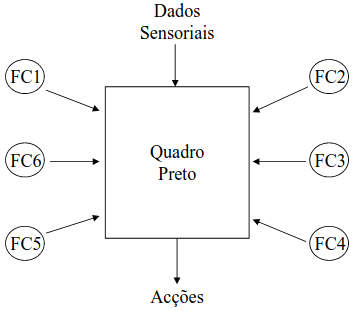
\includegraphics[scale=0.4]{13}
\end{center}

\pagebreak

\subsubsection{Agentes deliberativos}

Contrariamente aos anteriores, executam as ações com base em \textbf{objetivos} ou \textbf{função de
utilidade}.

\begin{center}
  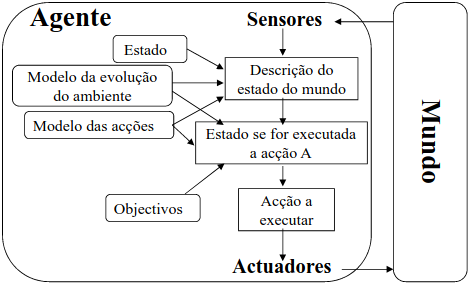
\includegraphics[scale=0.4]{14}
  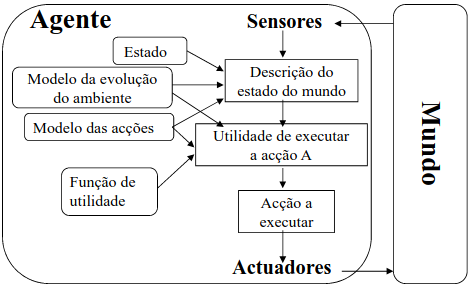
\includegraphics[scale=0.4]{15}
\end{center}

\begin{flushleft}
  \textbf{Primeira figura:} Agente deliberativo orientado a objetivos.

  \textbf{Segunda figura:} Agente deliberativo orientado por funções de utilidade.
\end{flushleft}

\begin{flushleft}
  \textbf{Nota:} A função de atividade é uma função que avalia a relevância de cada estado para o agente.
\end{flushleft}

\subsection{Propriedades do mundo de um agente}

Visto como se define um agente e os seus tipos, falta perceber como se caracteriza o seu
ambiente. Este pode apresentar várias propriedades.

\begin{itemize}
  \item \textbf{Acessibilidade -} O mundo é \textbf{acessível} se os sensores do agente tem acesso a toda a informação sobre o ambiente
  (descrição completa), ou pelo menos a toda a informação relevante.
  para o processo de escolha das ações (\textbf{efetivamente acessível}).
  \item \textbf{Determinismo -} Se o estado resultante da
  execução de uma ação é apenas e totalmente determinado pelo estado atual e pelos efeitos esperados
  da ação.
  \item \textbf{Munudo episódico -} Cada episódio de perceção-ação é totalmente indepente dos outros.
  \item \textbf{Dinamismo -}  O mundo é \textbf{dinâmico} se o seu estado pode mudar
  enquanto o agente delibera; caso contrário, o mundo diz-se \textbf{estático}.
  \item \textbf{Continuidade -} o mundo é \textbf{continuo} quando a evolução do estado do
  mundo é um processo continuo ou sem saltos; caso contrário o mundo
  diz-se \textbf{discreto}.
\end{itemize}

\begin{flushleft}
  \textbf{Exemplo:} Um agente táxi opera num ambiente dinâmico, enquanto que um agente que jogue palavras-cruzadas opera num
  ambiente estático.
  Para um agente carro de condução autónoma, a estrada é um ambiente contínuo. Já para um agente que jogue xadrez,
  o tabuleiro é um ambiente discreto.
\end{flushleft}

\pagebreak

\subsubsection{Mundo de um agente: Exemplos}

\begin{center}
  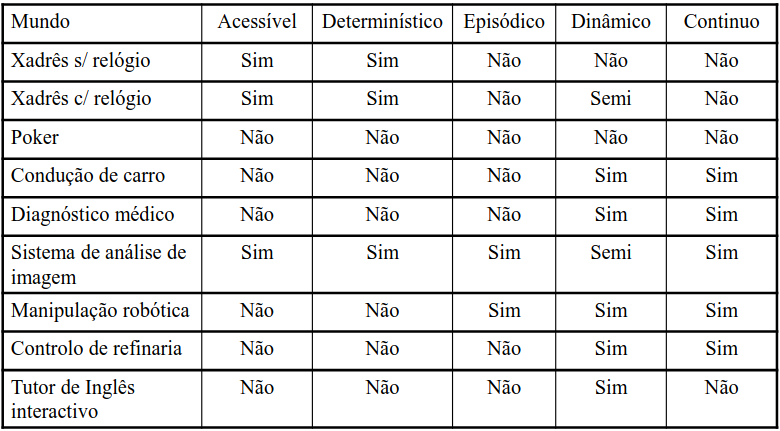
\includegraphics[scale=0.35]{16}
\end{center}

\subsection{Arquiteturas de agentes}

\subsubsection{Subsunção}

\begin{center}
  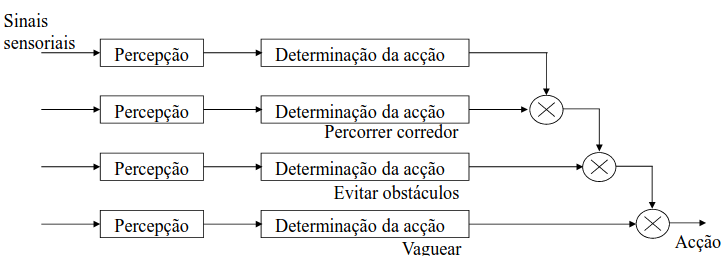
\includegraphics[scale=0.35]{17}
\end{center}

Esta arquitetura procura estabelecer a ligação entre a perceção e a ação a vários níveis,
organizados em camadas, criando agentes com comportamento simultâneamente reativo e
deliberativo.

\vspace{2mm}

A camada mais baixa é a mais reativa, diminuindo a reatividade e aumentando o peso da
componente deliberativa à medida que se sobe nas camadas. A ação do agente resulta da fusão das
decisões das várias camadas

\subsubsection{Três torres}

\begin{center}
  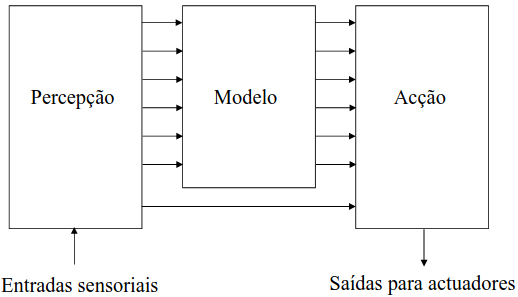
\includegraphics[scale=0.33]{18}
\end{center}

O processo de \textbf{tomada de decisão é simbólico} e feito a partir de um modelo,
mas tem \textbf{algumas ações reativas}.

\pagebreak

\subsubsection{Três camadas}

\begin{center}
  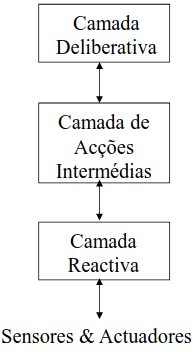
\includegraphics[scale=0.35]{19}
\end{center}

Para além das camadas deliberativas e reativas tem uma \textbf{camada de ações intermédias},
que é o intermediário entre as duas, produzindo uma alteração qualitativa no estado do
mundo.

\subsubsection{CARL}

\begin{center}
  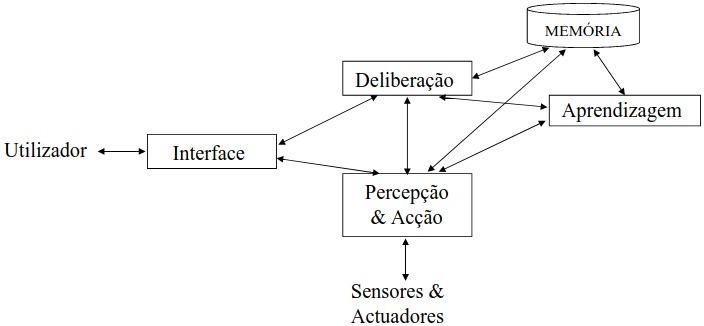
\includegraphics[scale=0.35]{20}
\end{center}

Esta arquitetura (anos 2000) veio introduzir dois novos conceitos:

\begin{itemize}
  \item \textbf{Interfaces -} Facilitam a interação por pessoas não especializadas;
  \item \textbf{Aprendizagem -} Para funcionar num ambiente humano não estruturado vai ter de aprender para se ir
  adapatando às condições do mundo real. Está assente em \textbf{memória}.
\end{itemize}

\section{Representação do conhecimento}

Para poderem tomar decisões, os agentes (especialmente os deliberativos) precisam de ter
algum conhecimento sobre o mundo em que se inserem.

\subsection{Redes Semânticas}

As \textbf{redes semânticas} são representações gráficas do conhecimento que facilitam a legibilidade
As redes semânticas podem ser tão expressivas quanto
a lógica de primeira ordem

\pagebreak

\subsubsection{Tipos de Relções}

\begin{itemize}
  \item Sub-tipo (ou sub-conjunto ou ainda sub-classe): $A \subset B$
  \item Membro (ou instância) de: $A \in B$
  \item Relação objeto-objeto: $R(A, B)$
  \item Relação conjunto-objeto: $\forall x x \in A \rightarrow R(x, B)$
  \item Relação conjunto-conjunto: $\forall x x \in A \rightarrow \exists (y \in B \wedge R(x, y))$
\end{itemize}

\subsubsection{Exemplo}

\begin{center}
  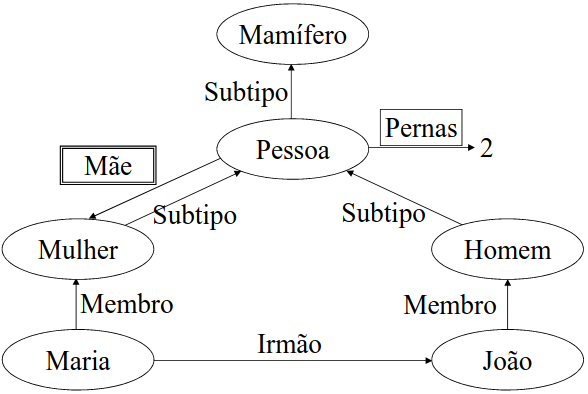
\includegraphics[scale=0.35]{21}
\end{center}

\subsubsection{Herança}

A herança pode ser representada em relações de \textbf{sub-tipo}, herdando todas as propriedades
dos tipos mais abstratos dos quais descende, ou de \textbf{instância}, herdando as todas as
propriedades do tipo a que pertence.
Aplica-se um \textbf{raciocínio não monotónico} devido ao estabelecimento dos \textbf{valores por defeito},
propriedades comuns a todos os membros desse tipo e do \textbf{cancelamento de herança}, que
ocorre quando um sub-tipo altera um valor por defeito herdado de um tipo do qual descende.

\subsubsection{Métodos e Demónios}

Normalmente, por razões computacionais, usam-se redes
semânticas bastante menos expressivas do que a lógica de primeira
ordem, deixando-se de lado a \textbf{negação}, a \textbf{disjunção} e a \textbf{quantificação}.

Em contra-partida, nomeadamente nos chamados sistemas de
frames, usam-se métodos e demónios:
\begin{itemize}
  \item \textbf{Métodos} - têm uma semântica similar à da programação orientada por objectos.
  \item \textbf{Demónios} - são procedimentos cuja execução é disparada automáticamente
  quando certas operações de leitura ou escrita são efetuadas.
\end{itemize}

\pagebreak

\subsection{UML / Diagramas de Classes}

Na linguagem gráfica UML (Unified Modelling Language), os
diagramas de classes definem as \uline{relações existentes entre as
diferentes classes} de objetos num dado domínio.
\begin{itemize}
  \item \textbf{Classe} - Descrição de um conjunto de objetos que partilham os mesmos
  atributos, operações, relações e semântica; estes objetos podem ser físicos
  ou conceituais.
  \item \textbf{Atributo} - Uma propriedade de uma classe.
  \item \textbf{Operação (ou método)} - implementação de um serviço.
  \item \textbf{Instância} - Um objeto que pertence a uma classe.
\end{itemize}

\begin{center}
  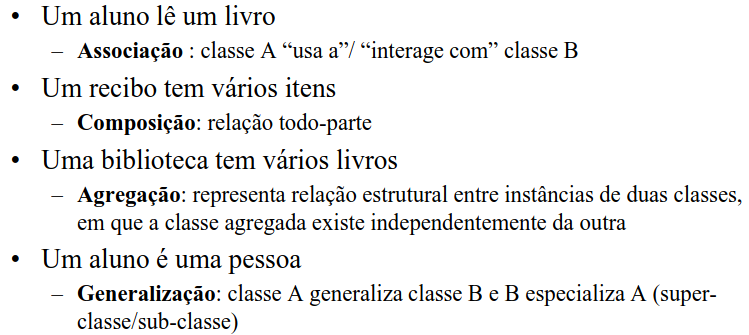
\includegraphics[scale=0.35]{22}
\end{center}

\begin{center}
  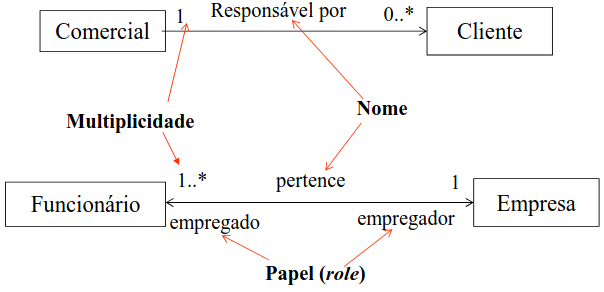
\includegraphics[scale=0.35]{23}
  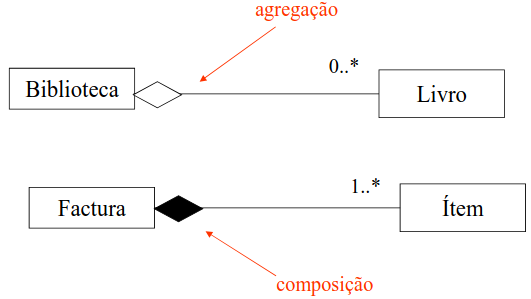
\includegraphics[scale=0.35]{24}
\end{center}

\subsection{Redes semânticas vs UML}

\begin{center}
  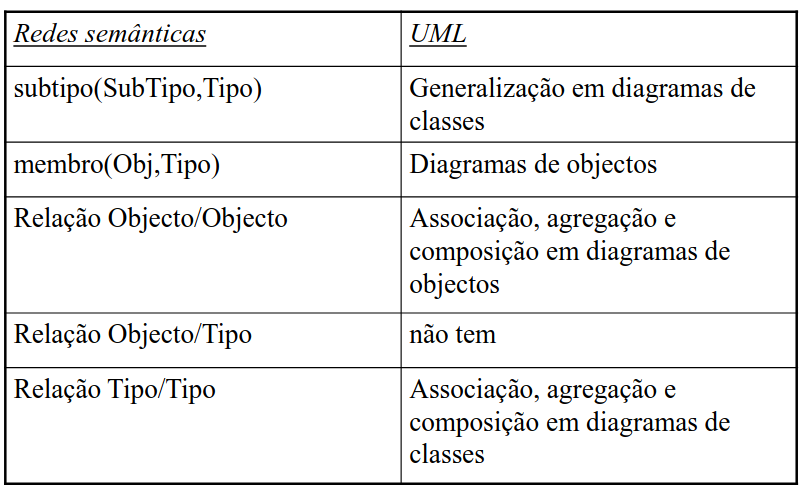
\includegraphics[scale=0.3]{25}
\end{center}

\pagebreak

\subsection{Indução versus Dedução}

A \textbf{dedução} permite a partir de um conjunto de permissas consideradas verdadeiras, por
mecanismos de inferências lógica, tirar conlusões verdadeiras.

No entanto, para adquirir conhecimento novo é necessário haver \textbf{indução}, ou seja, a
capacidade de inferir regras gerais a partir de observações concretas.

A dedução permite inferir casos particulares a partir de regras gerais, enquanto que
a indução permite inferir regras gerais a partir de casos particulares.

\subsubsection{Exemplo de Indução}

\begin{flushleft}
  Casos conhecidos:
  \begin{itemize}
    \item O gato Tareco gosta de leite;
    \item O gato Ozzy gosta de leite;
  \end{itemize}

  \uline{Regra inferida}: Os gatos (normalmente) gostam de leite.

  Nas redes semânticas, a indução pode ser vista como uma "herança de baixo para cima".
\end{flushleft}

\subsection{Lógicas}

Uma lógica tem:
\begin{itemize}
  \item \textbf{Sintaxe} - descreve o conjunto de frases ou fórmulas que é possível
  escrever (WFF - Well Formed Formulas);
  \item \textbf{Semântica} - estabelece a relação entre as frases escritas nessa
  linguagem e os factos que representam;
  \item \textbf{Regras de Inferência} - permitem manipular as frases, gerando
  umas a partir das outras; as regras de inferência são a base do
  processo de raciocínio.
\end{itemize}

\subsubsection{Lógica Proposicional}

A \textbf{lógica proposicional} é baseada em proposições, frases declarativas que podem ser
\textbf{verdadeiras ou falsas}, que podem ser representadas por \uline{variáveis proposicionais} que tomam o
seu valor de verdade. As fórmulas são compostas por uma ou mais variáveis proposicionais
ligadas por \uline{conectivas lógicas}.

\vspace{2mm}

\begin{flushleft}
  \textbf{Exemplo:} As proposições não dependem da interpretação, uma vez que, contrariamente aos predicados, as proposições não
  têm argumentos. "A neve é branca.” é uma proposição, que é verdadeira.
\end{flushleft}

\pagebreak

\subsubsection{Lógica de Primeira Ordem}

Em contraste temos a \textbf{lógica de primeira ordem}, onde há uma distinção entre os objetos e as
relações (predicados).

Além de variáveis, usadas para representar termos não especificados e constantes escalares,
os objetos podem ainda tomar a forma de \uline{expressões funcionais}, que se formam pela
aplicação de uma função aos seus argumentos. Os objetos podem ser considerados como
expressões funcionais cujo núemro de argumentos é zero.

O \uline{nome da relação aplica-se sempre ao seu primeiro elemento} (argumento). Os seus
argumentos só podem ser termos (nunca relação de relação).

\begin{flushleft}
  \textbf{Exemplo:} Potencia(4, 3) é uma \textbf{expressão funcional}.

  Pai(Rui, João) é um \textbf{predicado}. 
\end{flushleft}

\subsection{Conectivas Lógicas (LP, LPO)}

Comuns às duas lógicas abordadas, servem para \uline{combinar frases lógicas elementares} por
forma a obter frases mais complexas.

\begin{itemize}
  \item \textbf{Conjunção} - $p \wedge q$
  \item \textbf{Disjunção} - $p \vee q$
  \item \textbf{Implicação} - $p \rightarrow q$
  \item \textbf{Negação} - $\neg p$
\end{itemize}

\subsection{Variáveis, Quantificadores (LPO)}

Para quantificar as variáveis da lógica de primeira ordem temos os quantificadores universais e
os quantificadores existenciais.

\begin{itemize}
  \item \textbf{Quantificador universal} - $\forall x$.
  \begin{itemize}
    \item $\forall x A \equiv$ "Qualquer que seja x, a fórmula A é verdadeira"
  \end{itemize}
  \item \textbf{Quantificador existencial} - $\exists x$
  \begin{itemize}
    \item $\exists x A \equiv$ "Existe um x, para o qual a fórmula A é verdadeira"
  \end{itemize}
\end{itemize}

Se A é uma fórmula bem formada (FBF), então a sua quantificação também é uma FBF.

\pagebreak

\subsection{Gramáticas (LPO)}

\begin{center}
  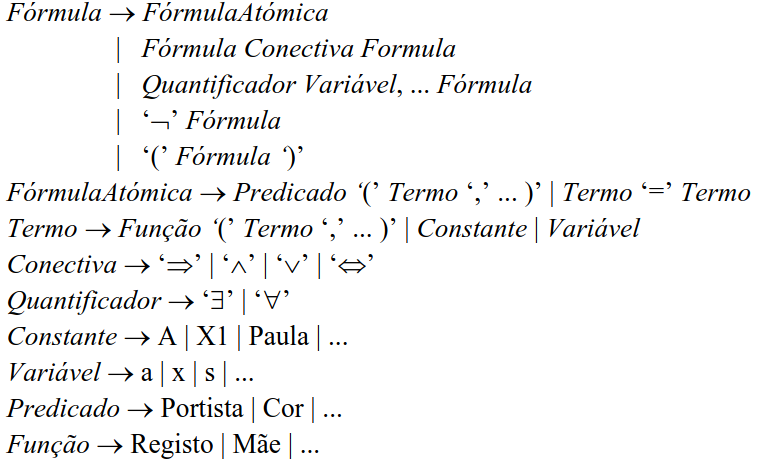
\includegraphics[scale=0.35]{26}
\end{center}

\subsubsection{Exemplo}

\begin{center}
  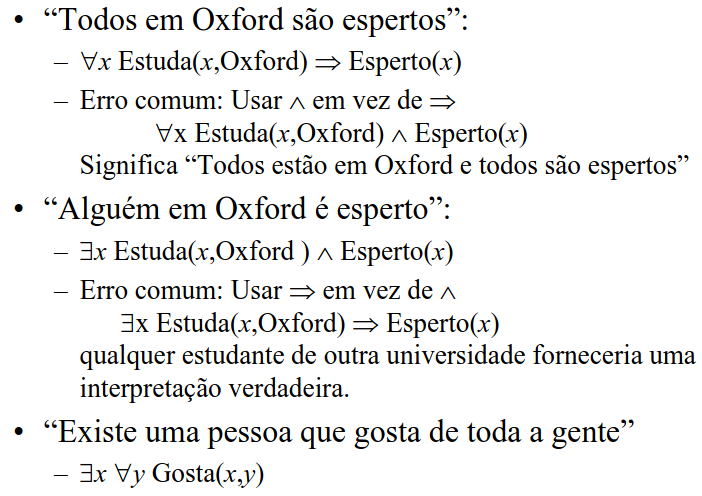
\includegraphics[scale=0.35]{27}
\end{center}

\subsection{Interpretações em Lógica Proposicional}

Na lógica proposicional, a interpretação de uma fórmula é a atribuição de valores de verdade
ou falsidade às várias proposições que nela ocorrem. \textbf{$A \wedge B$}  tem quatro interpretações possíveis que resultam da combinação dos valores de verdade e
falsidade de A e B.

\begin{itemize}
  \item \textbf{Satisfatibilidade} - Uma interpretação satisfaz uma fórmula
  sse a fórmula toma o valor "verdadeiro" para essa
  interpretação.
  \item \textbf{Modelo de uma fórmula} - uma interpretação que satisfaz
  essa fórmula.
  \item \textbf{Tautologia} - uma fórmula cujo valor é "verdadeiro" em
  qualquer interpretação. 
\end{itemize}

\pagebreak

\subsection{Interpretações em Lógica de Primeira Ordem}

Na \textbf{lógica de primeira ordem}, a interpretação de uma fórmula é o estabelecimento de uma
correspondência entre as constantes que ocorrem na fórmula e os objetos do mundo, funções e
relações que essas contantes representam.

\subsection{Regras de Substituição}

Estas regras permitem substituir uma fórmula por outra equivalente.
São válidas tanto para a lógica proposicional como para a lógica de primeira ordem.

\begin{center}
  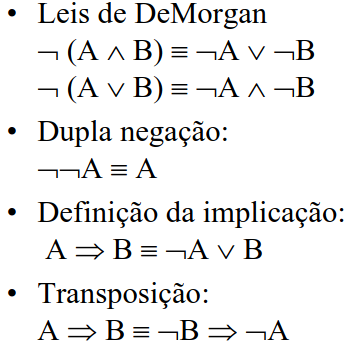
\includegraphics[scale=0.35]{28}
  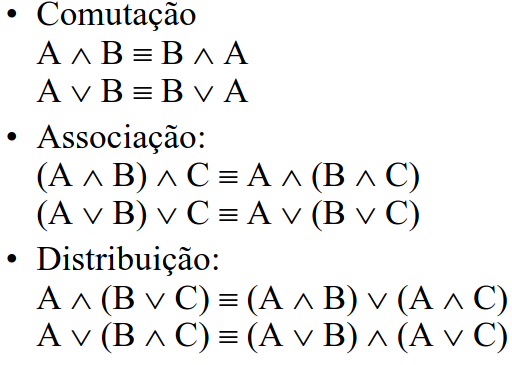
\includegraphics[scale=0.35]{29}
\end{center}

Leis de DeMorgan generalizadas (estas são específicas
da lógica de primeira ordem):

\begin{center}
  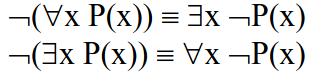
\includegraphics[scale=0.35]{30}
\end{center}

\subsection{CNF e Forma Clausal}

Uma fórmula na \textbf{forma normal conjuntiva} (CNF) é uma fórmula que consiste de uma
conjunção de cláusulas.

\begin{flushleft}
  \textbf{Cláusula -} fórmula que consiste de uma
  disjunção de literais.

  \textbf{Literal -} fórmula atómica (literal positivo) ou a
  negação de uma fórmula atómica (literal negativo). Na LP uma
  fórmula atómica é uma proposição.

  \textbf{Forma Causal -} representação de uma fórmula CNF através do conjunto
  das respetivas cláusulas.
\end{flushleft}

\begin{flushleft}
  \textbf{Exemplo:}

  \uline{Literal} - $p$ ou $\neg p$

  \uline{Claúsula} - $I1 \vee I2$ $\vee$ \dots

  \uline{CNF} - c1 \& c2 \& \dots CNF

  \uline{Forma Causal} - [c1, c2, \dots]
\end{flushleft}

\pagebreak

\subsubsection{Conversão de uma Fórmula
Proposicional para CNF e forma clausal}

\begin{center}
  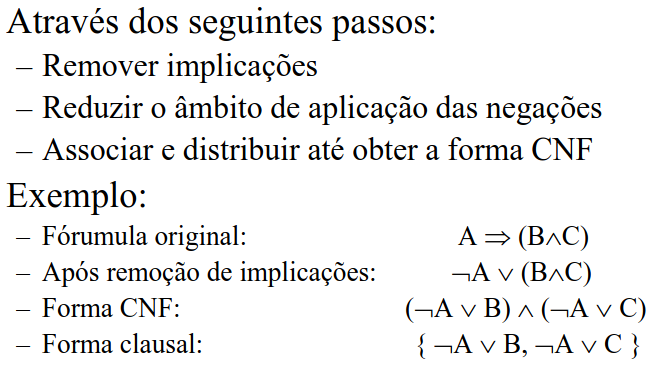
\includegraphics[scale=0.35]{31}
\end{center}

\subsubsection{Conversão para forma clausal em
Lógica de Primeira Ordem}

\begin{center}
  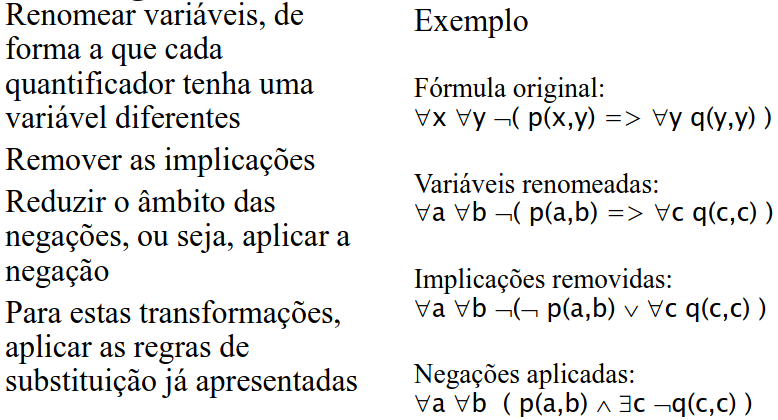
\includegraphics[scale=0.25]{32}
  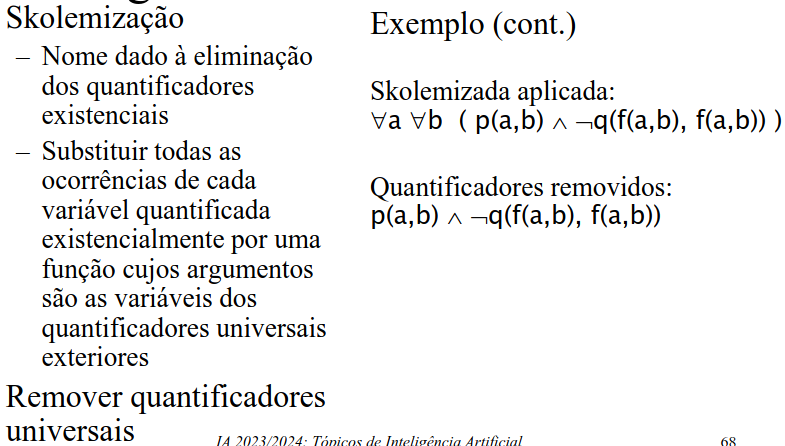
\includegraphics[scale=0.25]{33}

  \vspace{2mm}
  
  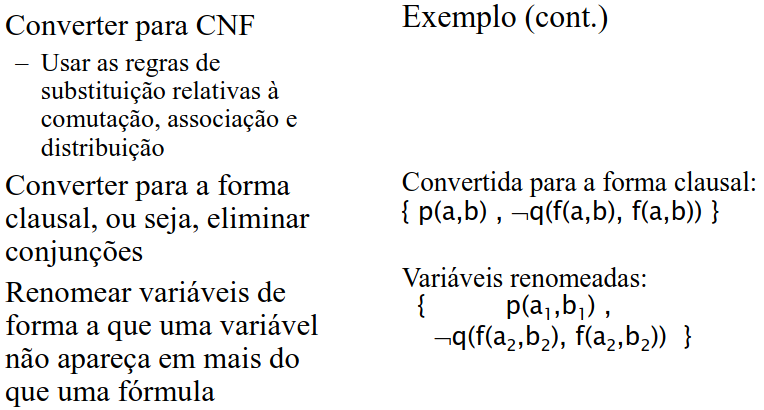
\includegraphics[scale=0.3]{34}
\end{center}

\pagebreak

\subsection{Lógica - Regras de Inferência}

\begin{center}
  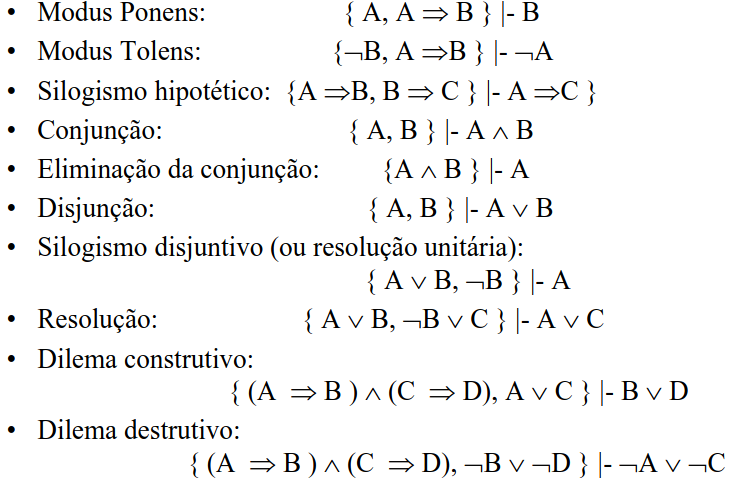
\includegraphics[scale=0.35]{35}
\end{center}

\subsubsection{LPO - Regras de Inferência específicas}

\begin{center}
  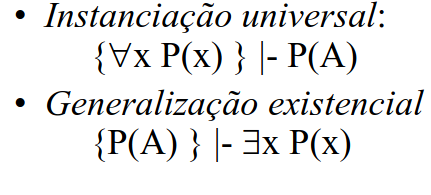
\includegraphics[scale=0.3]{36}
\end{center}

\subsection{Consequências lógicas e provas}

A regras de inferência permitem-nos obter consequências lógicas (A) a partir de um conjunto
de fórmulas ( $\Delta$ = { A1, \dots, An }), representada esta noção por $\vDash$.

\[ \Delta \vDash A \]

Esta consequência é obtida se A tomar o valor verdadeiro em \textbf{todas as interpretações} para as
quais cada uma das fórmulas em $\Delta$ toma também o valor \textbf{verdadeiro}.

\vspace{2mm}

A \textbf{prova} de uma fórmula $A_n$ é dada pela sequência de fórmulas $\Delta = \{ A_1, \dots, A_n \}$ tal que cada $A_i$
pode ser inferida a partir das fórmulas anteriores $A_1, \dots, A_{i-1}$. Neste caso, escreve-se:

\[ \Delta \vdash A_n \]

\pagebreak

\subsection{Correção, Completude}

\begin{flushleft}
  \textbf{Correção -} Diz-se que um conjunto de regras de
  inferência é correto se \textbf{todas as fórmulas que gera são
  consequências lógicas}.

  \vspace{2mm}

  \textbf{Completude -} Diz-se que um conjunto de regras de
  inferência é completo se \textbf{permite gerar todas as
  consequências lógicas}.
\end{flushleft}

Um sistema de inferência correto e completo permite tirar consequências lógicas sem ter que analisar caso a
caso as várias interpretações.

\subsection{Metateoremas}

\vspace{2mm}

\begin{center}
  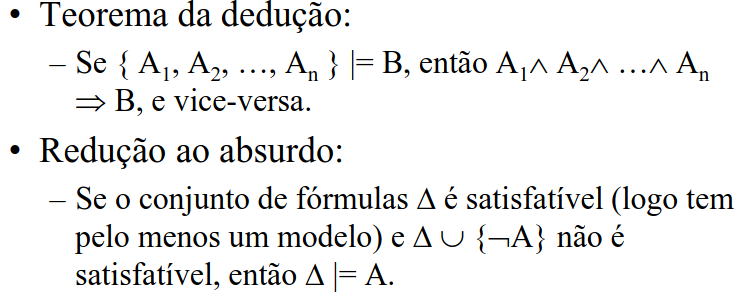
\includegraphics[scale=0.3]{37}
\end{center}

\subsection{Resolução não é Completa}

A resolução é uma regra de inferência correta
(gera fórmulas necessáriamente verdadeiras)

\[ \{ A \wedge B, \neg B \wedge C \} \vdash A \wedge C \]

A resolução não é completa. Exemplo, a resolução não consegue derivar a
seguinte consequência lógica:

\[ \{ A \vee B \} \vDash A \wedge B \]

\subsection{Refutação por Resolução}

Este é um \textbf{mecanismo de inferência completo}, usa-se a resolução para provar que a negação da
consequência lógica é inconsistente com a premissa (metateorema da redução ao absurdo). Para tal,
basta derivar Falso.

No exemplo dado, prova-se que $(A \wedge B) \wedge \neg (A \vee B)$ é inconsistente
(basta mostrar que é possível derivar a fórmula "Falso").

\subsubsection{Passos}

\begin{itemize}
  \item Converter a premissa e a negação da consequência lógica
  para um conjunto de cláusulas.
  \item Aplicar a resolução até obter a cláusula vazia.
\end{itemize}

\pagebreak

\subsubsection{Substituições, Unificação}

\begin{center}
  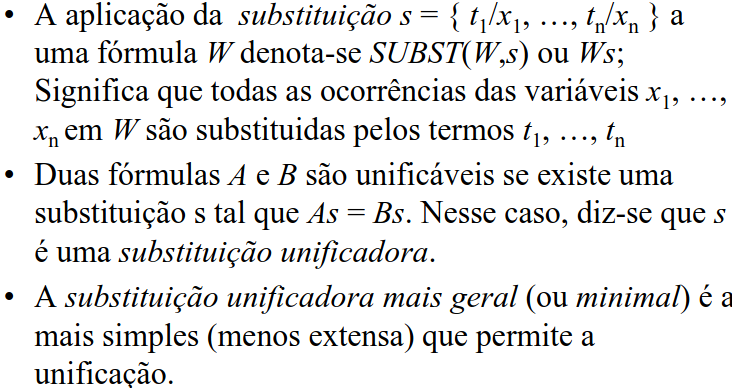
\includegraphics[scale=0.3]{38}
\end{center}

\subsubsection{Resolução e Refutação
na Lógica de Primeira Ordem}

\begin{center}
  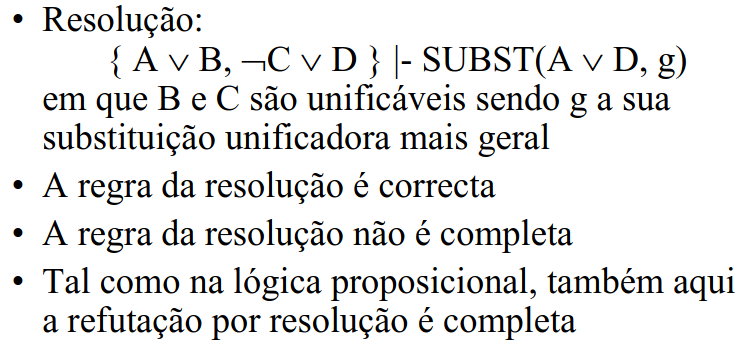
\includegraphics[scale=0.3]{39}
\end{center}

\subsection{Resolução com Claúsulas de Horn}

A \textbf{refutação por resolução} é correta e completa, mas apesar de melhor que avaliar todas as
interpretações da inferência, continua a ser pouco eficiente.

\begin{flushleft}
  \textbf{Nota:} Para várias cláusulas com muitos literais em cada uma vão haver múltiplos casos em que a resolução pode ser
  aplicada entre um literal e outros de outras formulas, o que vai gerar uma explosão de casos e um problema
  tendencialmente mais difícil de resolver com o aumento do seu tamanho.
\end{flushleft}

Uma cláusula de Horn é uma cláusula que tem
no máximo um literal positivo, como: $A$, $\neg A \vee B$, $\neg A \vee B \vee \neg C$ e
$\neg A \vee \neg B$.

Existem algoritmos de dedução baseados em
cláusulas de Horn cuja complexidade temporal
é linear.

\begin{flushleft}
  \textbf{Exemplo:} $\neg A \vee B \vee \neg C$ (=) $A \wedge C \rightarrow B$
\end{flushleft}

\begin{flushleft}
  \textbf{Nota:} O problema da combinatória da refutação por resolução vai ser minimizado, uma vez nas cláusulas de Horn cada
  cláusula vai ter menos possibilidades de resolução. O seu literal positivo pode ser resolvido com um negativo noutra
  fórmula e o inverso para os seus literais negativos.
\end{flushleft}

Estas cláusulas permitem a aplicação de algoritmos com \uline{complexidade temporal linear}.

\section{Representação do conhecimento}


\end{document}